\documentclass[11pt]{article}

\usepackage[margin=1in]{geometry}
\usepackage{amsmath,amssymb,amsfonts}
\usepackage{bm}
\usepackage{booktabs}
\usepackage{graphicx}
\usepackage{hyperref}
\usepackage{enumitem}
\usepackage{algorithm}
\usepackage{algpseudocode}
\usepackage{xcolor}
\graphicspath{{figures/}}

\hypersetup{colorlinks=true, linkcolor=blue, citecolor=blue, urlcolor=blue}

\title{\textbf{Learning-Based Digital-Twin Placement and Resource Allocation\\
for Integrated Satellite--Terrestrial Networks:\\
A Multi-Agent Reinforcement Learning Framework}}

\author{SatTwin Project --- Progress Report}
\date{\today}

\begin{document}

\maketitle

\begin{abstract}
Non-terrestrial networks (NTNs) built on low Earth orbit (LEO) constellations are
a cornerstone of the emerging sixth-generation (6G) communication vision, promising
ubiquitous, high-throughput connectivity across terrestrial, aerial, and space
segments. Managing such networks in real time requires a \emph{network digital
twin} (NDT): a synchronized virtual replica of each physical satellite that
supports low-latency monitoring, prediction, and control. A central operational
problem is deciding, at every control epoch, \emph{where each satellite's digital
twin should be hosted} among a set of geographically distributed ground stations,
and \emph{how the finite radio and computing resources of each ground station
should be shared} among the twins it serves. This report formulates that joint
placement-and-allocation problem as a partially observable, time-coupled
Markov decision process under realistic operational constraints---finite gateway
capacity, congestion-dependent service, handover signaling cost, on-board energy
budgets with orbital eclipse cycles, delayed telemetry feedback, and stochastic
traffic demand. We develop a multi-agent reinforcement learning (MARL) controller
based on centralized-training / decentralized-execution proximal policy
optimization, with a graph-neural-network state encoder for topological
generalization and a hybrid discrete--continuous action head for joint gateway
selection and bandwidth allocation. We describe the system model, the learning
architecture, the evaluation methodology against classical control heuristics, and
the current experimental status.
\end{abstract}

\section{Motivation}
\label{sec:motivation}

Future 6G systems are expected to deliver seamless service well beyond dense urban
cells, extending reliable connectivity to aerial, maritime, rural, and remote
environments through the tight integration of terrestrial infrastructure with
non-terrestrial platforms such as LEO satellite constellations and high-altitude
platform stations. LEO constellations, in particular, provide near-global coverage
with comparatively low propagation delay, but they introduce a distinctive control
challenge: the space segment is intensely dynamic. Satellites move at orbital
velocities of several kilometres per second, the set of ground stations visible to
a given satellite changes continuously, link quality varies with elevation angle
and weather, and user traffic demand fluctuates on both diurnal and short
timescales.

To operate such a network reliably, operators increasingly rely on a
\emph{network digital twin}: a continuously synchronized virtual model of the
physical system that mirrors each satellite's state and supports fault diagnosis,
what-if analysis, resource optimization, and closed-loop control. The fidelity and
usefulness of a digital twin depend directly on the \emph{synchronization latency}
between each physical satellite and its virtual counterpart, which in turn depends
on where the twin is hosted in the terrestrial ground-station network. As a
satellite traverses its orbit, the ground station that minimizes this latency
changes, so the twin must be \emph{migrated} between hosting stations over time.

Two features make this more than a simple ``assign each satellite to its nearest
ground station'' problem, and they are the crux of why a learned controller is
warranted:

\begin{enumerate}[leftmargin=*]
  \item \textbf{Coupling and contention.} Ground stations have finite radio and
  compute capacity. Because many satellites become visible to the same
  well-placed station simultaneously, independent, per-satellite decisions
  systematically overload popular stations, degrading service for all twins
  hosted there. The optimal decision for one satellite depends on the decisions
  taken for all others---a coupling that per-entity rules cannot resolve.

  \item \textbf{Temporal state and long-horizon consequences.} The system carries
  persistent state that accumulates across control epochs. Undelivered data
  builds up in on-board buffers and is lost if a buffer overflows; each twin
  migration consumes signaling resources and on-board energy; and energy is
  replenished only while a satellite is illuminated by the Sun, being unavailable
  during orbital eclipse. A decision that is locally attractive at one epoch (for
  instance, migrating aggressively to shave instantaneous latency) can be
  globally harmful several epochs later (buffer overflow, exhausted batteries).
  Effective control therefore requires reasoning over a horizon, not greedily
  optimizing the current epoch.
\end{enumerate}

These characteristics---partial observability through delayed feedback, strong
inter-agent coupling under shared capacity, and long-horizon temporal
dependencies through persistent physical state---are precisely the conditions
under which sequential decision-making via reinforcement learning is the natural
methodology. This motivates the framework developed in the remainder of this
report.

\section{System Model}
\label{sec:model}

We consider a downlink integrated satellite--terrestrial network in which a LEO
constellation of $K$ satellites is served by a set $\mathcal{G}$ of geographically
distributed ground stations (gateways), coordinated by a central network control
center. Each satellite $k \in \mathcal{K} = \{1,\dots,K\}$ is associated with a
digital twin that must be hosted at exactly one gateway at each discrete control
epoch $t \in \{0,1,2,\dots\}$ of duration $\Delta t$.

\subsection{Orbital and topological dynamics}
Satellite positions evolve according to Walker-constellation orbital mechanics;
the position of satellite $k$ at epoch $t$ is a deterministic function
$\bm{p}_k(t)$ of its orbital elements. A gateway $g \in \mathcal{G}$ is reachable
from satellite $k$ only when the satellite is above a minimum elevation angle
$\varepsilon_{\min}$ relative to the gateway. Inter-satellite links (ISLs) connect
neighbouring satellites, so a twin hosted at a gateway not directly visible to its
satellite is reached over a multi-hop path. The end-to-end propagation latency
$\ell_{k,g}(t)$ between satellite $k$ and a candidate host gateway $g$ is computed
as the shortest weighted path in the time-varying network graph
$\mathcal{N}(t)$ whose edges (ISL, ground, and terrestrial links) are weighted by
propagation delay. Because the gateway network is geographically clustered over
populated land masses, a satellite periodically enters a \emph{coverage gap}---an
interval over ocean or polar regions during which no gateway is directly visible
and the twin is reachable only over long multi-hop paths, if at all. These gaps
are deterministic functions of orbital geometry and therefore, in principle,
predictable from the constellation state.

\subsection{Link quality and capacity}
The instantaneous quality of the access link is elevation dependent: low-elevation
links incur an additional latency penalty reflecting reduced signal quality, and
are further degraded by time-correlated atmospheric fading (rain fade) modelled as
a two-state Gilbert process per gateway. Each gateway $g$ has a finite hosting
capacity $C_g$. Rather than a hard admission block, we adopt a \emph{soft-capacity}
model in which additional twins may be admitted beyond nominal capacity but incur
a convex congestion penalty
\begin{equation}
  c_g(t) \;=\; c_0 \left( \frac{n_g(t)}{C_g} \right)^{\gamma}
  \;+\; d_g(t)\left(\tfrac{1}{2} + \tfrac{n_g(t)}{C_g}\right),
  \label{eq:congestion}
\end{equation}
where $n_g(t)$ is the number of twins hosted at $g$, $\gamma>1$ controls the
sharpness of congestion growth, and $d_g(t)$ is the exogenous traffic demand at
gateway $g$. The demand $d_g(t)$ follows a predictable diurnal wave whose phase is
offset by gateway longitude, plus stochastic surges of random onset and duration.
The effective latency experienced by twin $k$ hosted at $g$ is
$\tilde{\ell}_{k,g}(t) = \ell_{k,g}(t) + c_g(t) + h_k(t)$, where $h_k(t)$ is a
transient handover penalty incurred for a fixed number of epochs after a
migration to account for link re-establishment.

\subsection{Data queues and delivered rate}
Each satellite accumulates traffic in an on-board buffer of capacity $B$. Let
$q_k(t)$ denote the queue backlog of satellite $k$. At each epoch, new data arrives
according to a bursty per-satellite process $a_k(t)$, and data is drained at a
service rate determined by the \emph{shared} throughput of its host gateway:
\begin{equation}
  q_k(t{+}1) \;=\; \min\!\Big\{\, B,\; \big[\, q_k(t) + a_k(t) - s_k(t) \,\big]^+ \Big\},
  \qquad
  s_k(t) = \frac{S_g}{n_g(t)},
  \label{eq:queue}
\end{equation}
where $S_g$ is the gateway service capacity shared equally (in the baseline) among
the $n_g(t)$ co-hosted twins, and $[\cdot]^+$ denotes the positive part. Any
backlog exceeding $B$ is irrecoverably \emph{dropped}. The delivered data rate to
satellite $k$ follows a Shannon-type expression on the effective signal-to-noise
ratio $\mathrm{SINR}_k(t) \propto 1/\tilde{\ell}_{k,g}(t)$, scaled by the fraction
of gateway bandwidth allocated to the link:
\begin{equation}
  R_k(t) \;=\; W_{k}(t)\,\log_2\!\big(1 + \mathrm{SINR}_k(t)\big),
  \qquad
  W_k(t) = W_g \cdot \frac{w_k(t)}{\sum_{j \in \mathcal{S}_g} w_j(t)},
  \label{eq:rate}
\end{equation}
where $\mathcal{S}_g$ is the set of twins hosted at $g$, $W_g$ is the gateway's
total bandwidth, and $w_k(t) \ge 0$ is a per-twin bandwidth weight. Setting all
weights equal recovers a proportional-fair split; the weights are a control
variable (Section~\ref{sec:mdp}).

\subsection{Data freshness and delivery deadlines}
Traffic is not merely rate-limited but \emph{time-critical}. We track the age
$\alpha_k(t)$ of the oldest undelivered data in each satellite's buffer: the age
grows while the backlog cannot be drained and resets when service resumes. Data
that remains undelivered beyond a freshness deadline $\alpha_{\max}$ expires and is
irrecoverably lost:
\begin{equation}
  \text{if } \alpha_k(t) > \alpha_{\max}: \quad
  q_k(t) \rightarrow 0, \;\; \alpha_k(t) \rightarrow 0, \;\;
  \text{(backlog counted as expired loss)}.
  \label{eq:deadline}
\end{equation}
This Age-of-Information constraint fundamentally alters the control problem: it is
insufficient to eventually deliver data; it must be delivered \emph{in time}.
Combined with the coverage dynamics of Section~\ref{sec:model} (a satellite
periodically loses visibility of all gateways as it transits ocean and polar
regions), this rewards controllers that \emph{anticipate}---pre-positioning twins
and shaping bandwidth before an impending coverage gap or demand surge, rather than
reacting after a deadline has already been missed. A further consequence is
\emph{synchronized contention}: when many satellites regain gateway visibility
simultaneously, independent per-satellite decisions concentrate load on the same
newly-available gateways, causing correlated buffer overflow---a failure mode that
only coordinated, load-aware placement can avoid.

\subsection{Energy and eclipse}
Each satellite carries a battery of capacity $E_{\max}$ with state of charge
$e_k(t)$. Transmitting data and, more significantly, migrating a twin both consume
energy; energy is recharged at a fixed rate only when the satellite is in
sunlight, and not during the eclipse fraction of each orbit:
\begin{equation}
  e_k(t{+}1) \;=\; \min\!\Big\{ E_{\max},\;
  e_k(t) - \eta_{\mathrm{tx}}\,\tfrac{s_k(t)}{S_g}
  - \eta_{\mathrm{mig}}\,\mathbb{1}[\text{migrate}_k(t)]
  + \eta_{\mathrm{rec}}\,\mathbb{1}[\text{sunlit}_k(t)] \Big\}.
  \label{eq:energy}
\end{equation}
A satellite with a depleted battery cannot transmit, so its queue grows and
eventually overflows. Energy therefore couples the migration policy to
delivered rate over the orbital timescale.

\subsection{Delayed feedback}
The control center does not observe the instantaneous network state. Telemetry
(congestion, demand, queue, link quality) arrives with a feedback delay of $d$
epochs, so decisions at epoch $t$ are conditioned on state as of epoch $t-d$. This
renders the problem \emph{partially observable} and rewards a controller that can
anticipate the evolution of the predictable components of the state (orbital
geometry, diurnal demand) rather than merely reacting to stale measurements.

\section{Problem Formulation}
\label{sec:mdp}

We cast the joint twin-placement and resource-allocation problem as a
decentralized partially observable Markov decision process (Dec-POMDP), with one
agent per satellite digital twin. This framing aligns naturally with the physical
hierarchy: the central control center possesses global state and is used for
\emph{training}, while each twin acts on local observations for low-latency
\emph{execution}.

\paragraph{Agents.} Each satellite $k \in \mathcal{K}$ is an agent. Agents are
homogeneous and share a single policy network (parameter sharing), which allows
the learned controller to scale to and generalize across constellation sizes.

\paragraph{Observation.} At epoch $t$, agent $k$ observes a local feature vector
$o_k(t)$ comprising: its current (delayed) effective latency and a one-step
extrapolation; the candidate effective latencies to all reachable gateways; the
normalized load of each gateway; its normalized queue backlog $q_k(t)/B$; its
normalized battery level $e_k(t)/E_{\max}$; the time since its last migration; and
the identity of its current host. Latencies are normalized to a bounded range to
keep the representation well-conditioned.

\paragraph{Global state.} The centralized critic additionally observes the joint
twin-to-gateway assignment, all gateway loads and capacities, and all per-agent
latencies---information available only at the control center.

\paragraph{Action.} Each agent selects a \emph{hybrid} action
$a_k(t) = \big(g_k(t),\, w_k(t)\big)$, where $g_k(t) \in \{\text{stay}\} \cup
\mathcal{G}$ is a discrete host-gateway decision (remain, or migrate to a
reachable gateway), and $w_k(t) \in [w_{\min}, w_{\max}]$ is a continuous
bandwidth-request weight entering Eq.~\eqref{eq:rate}. A feasibility mask restricts
$g_k(t)$ to reachable gateways and to hosts within the soft-capacity limit.

\paragraph{Reward.} The team reward at epoch $t$ combines system-level
quality-of-service objectives with operational-cost penalties:
\begin{align}
  r(t) \;=\;\;
    &\; \lambda_{\mathrm{sum}}\, \textstyle\sum_{k} R_k(t)
     + \lambda_{\mathrm{min}}\, \min_{k} R_k(t)
     + \lambda_{\mathrm{fair}}\, J\big(\bm{R}(t)\big) \nonumber \\
    &- \lambda_{\mathrm{q}}\, \bar{q}(t)
     - \lambda_{\mathrm{drop}}\, D(t)
     - \lambda_{\mathrm{en}}\, F(t)
     - \lambda_{\mathrm{mig}}\, M(t),
  \label{eq:reward}
\end{align}
where $J(\cdot)$ is Jain's fairness index over the delivered rates
$\bm{R}(t)$, $\bar{q}(t)$ is the mean queue backlog, $D(t)$ is the volume of
dropped data (from both buffer overflow and deadline expiry,
Eq.~\eqref{eq:deadline}), $F(t)$ is the number of energy-depleted satellites, and
$M(t)$ is the number of migrations. The weights $\lambda$ encode the operator's
preference among throughput, fairness, weak-user protection, buffer health, data
freshness, energy sustainability, and control stability. Jain's fairness index for a rate
vector $\bm{R} = (R_1,\dots,R_K)$ is
\begin{equation}
  J(\bm{R}) \;=\; \frac{\big(\sum_k R_k\big)^2}{K \sum_k R_k^2}\;\in\;(0,1],
\end{equation}
attaining its maximum when all delivered rates are equal.

\paragraph{Objective.} The controller seeks a policy $\pi_\theta$ maximizing the
expected discounted return $\mathbb{E}_{\pi_\theta}\big[\sum_{t} \gamma^t r(t)\big]$,
with discount factor $\gamma \in (0,1)$, subject to the feasibility mask and the
soft-capacity constraint. The discounting is essential: because queues, energy,
and handover costs accumulate, the value of an action is determined by its
\emph{future} consequences, not solely its immediate reward.

\section{Learning Architecture}
\label{sec:arch}

We adopt multi-agent proximal policy optimization (MAPPO) under the
centralized-training, decentralized-execution (CTDE) paradigm.

\subsection{Graph-based state encoding}
The time-varying network is naturally a heterogeneous graph with satellite,
gateway, and control-center nodes and ISL, ground, and terrestrial edges weighted
by propagation delay. We encode this graph with a message-passing graph neural
network (GNN) that produces a per-node embedding. Because message passing
aggregates over local neighbourhoods rather than fixed indices, the encoder is
\emph{inductive}: a policy trained on one constellation size can be applied,
without retraining, to a differently sized constellation---the basis for our
generalization study (Section~\ref{sec:eval}). A per-agent recurrent (gated)
encoder additionally summarizes each satellite's recent observation history, which
supports anticipation under the delayed-feedback model.

\subsection{Hybrid actor and centralized critic}
The shared actor consumes the fused per-agent representation (graph embedding,
temporal summary, and local scalar features) and emits a hybrid action
distribution: a masked categorical distribution over the discrete gateway choice
and a Gaussian (squashed to a bounded interval) over the continuous bandwidth
weight. The joint log-probability is the sum of the two component
log-probabilities, and PPO's clipped surrogate objective is applied to the joint
action. The centralized critic estimates the state value from the global state and
is used only during training; at execution each agent requires only its local
observation, respecting the low-latency requirement of the edge twins.

\subsection{Optimization}
Training uses clipped-surrogate policy updates with generalized advantage
estimation on the team return, a clipped value loss, an entropy regularizer for
exploration, and Kullback--Leibler-based early stopping for update stability.
Rollouts are collected in parallel across multiple workers to increase throughput.
Algorithm~\ref{alg:mappo} summarizes one training iteration.

\begin{algorithm}[t]
\caption{MAPPO training iteration (CTDE)}
\label{alg:mappo}
\begin{algorithmic}[1]
\State Collect parallel rollouts: for each epoch, encode observations, sample
hybrid actions under the feasibility mask, apply migrations and bandwidth weights,
advance the environment (queues, energy, demand, fading), and record team rewards
and the global state.
\State Compute generalized advantage estimates and value targets from the team
return.
\For{each epoch over minibatches}
  \State Evaluate joint action log-probabilities and entropy under the current
  policy.
  \State Update the actor by the clipped surrogate objective minus an entropy
  bonus; stop early if the KL divergence exceeds a threshold.
  \State Update the centralized critic by the clipped value loss.
\EndFor
\end{algorithmic}
\end{algorithm}

\section{Evaluation Methodology}
\label{sec:eval}

We evaluate the learned controller against a suite of classical control
strategies that represent the standard operational alternatives:
\begin{itemize}[leftmargin=*]
  \item \textbf{Nearest-gateway:} each twin is hosted at its lowest-effective-latency
  reachable gateway at every epoch.
  \item \textbf{Hysteresis (margin) control:} migration occurs only when a
  candidate gateway improves effective latency by more than a fixed margin,
  reducing handover churn.
  \item \textbf{Per-epoch optimal assignment:} a minimum-cost bipartite matching of
  twins to capacitated gateway slots, computed independently each epoch (a
  per-epoch, myopic optimum).
  \item \textbf{Static placement:} an initial feasible assignment held fixed.
  \item \textbf{Randomized feasible:} a stochastic feasibility-respecting policy
  serving as a lower reference.
\end{itemize}

All methods are evaluated in the identical environment with the same realistic
constraints. Reported metrics are the system-level quantities of
Eq.~\eqref{eq:reward}: aggregate delivered rate, worst-case (minimum) delivered
rate, Jain's fairness index, mean queue backlog and dropped-data volume, count of
energy-depleted satellites, and migration (handover) count. Beyond in-distribution
performance, we assess \emph{generalization} by training on one constellation and
evaluating zero-shot on a larger one, exploiting the inductive GNN encoder.

\subsection{Experimental setup}
The constellation follows a Walker configuration of low Earth orbit satellites at
$780$~km altitude with $86.4^\circ$ inclination, served by a geographically
clustered set of ground gateways with finite hosting capacity. Control proceeds in
discrete epochs; each training episode spans a full range of orbital and demand
phases so that coverage gaps, diurnal demand waves, eclipse cycles, and stochastic
surges are all exercised. The policy and centralized critic are optimized with the
CTDE MAPPO procedure of Algorithm~\ref{alg:mappo} using generalized advantage
estimation, clipped surrogate updates, value-target normalization, and an
annealed entropy regularizer. Unless otherwise noted, results are reported on the
constraint-rich environment of Section~\ref{sec:model} with all mechanisms active.

\section{Results and Discussion}
\label{sec:results}

We organize the evaluation around the operational objectives that distinguish a
horizon-aware controller from myopic alternatives: worst-user protection, rate
fairness, control (handover) overhead, overall multi-objective performance, and
cross-constellation generalization.

\subsection{Worst-user protection}
Figure~\ref{fig:minrate} tracks the minimum delivered rate across all satellites
over training. The learned policy raises the worst-served satellite's rate by
roughly threefold relative to its starting point and sustains it, whereas the
myopic baselines leave the weakest users starved at a near-zero floor. This
directly reflects the $\min_k R_k(t)$ term in the reward of
Eq.~\eqref{eq:reward}: rather than maximizing aggregate throughput at the expense
of the tail, the controller learns to protect the most disadvantaged links---the
behaviour operators require for service-level guarantees.

\begin{figure}[t]
  \centering
  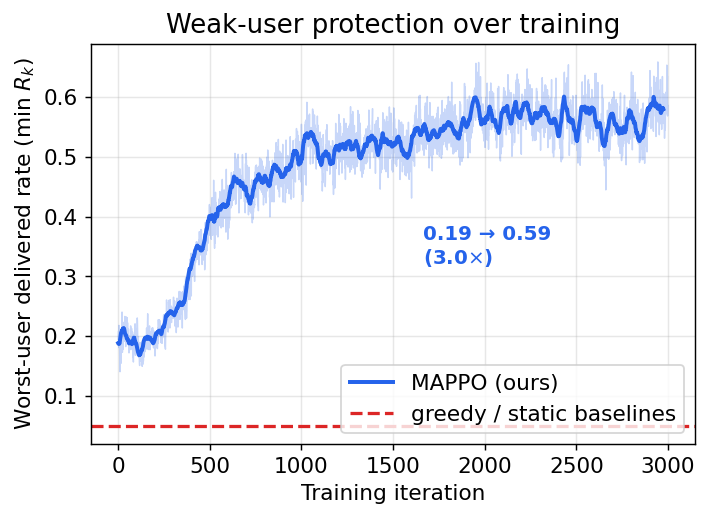
\includegraphics[width=0.62\linewidth]{fig1_min_rate.png}
  \caption{Worst-user delivered rate ($\min_k R_k$) over training. The learned
  controller improves the weakest satellite's rate approximately threefold and
  sustains it, far above the myopic-baseline floor.}
  \label{fig:minrate}
\end{figure}

\subsection{Rate fairness}
Figure~\ref{fig:fairness} reports Jain's fairness index over training. The
controller converges to a fairness index substantially above the nearest-gateway
baseline, indicating a markedly more equitable distribution of delivered rate
across the constellation. Because gateway bandwidth is shared, fairness cannot be
achieved by any single satellite acting alone; it emerges from the coordinated,
capacity-aware allocation that the centralized-critic training induces.

\begin{figure}[t]
  \centering
  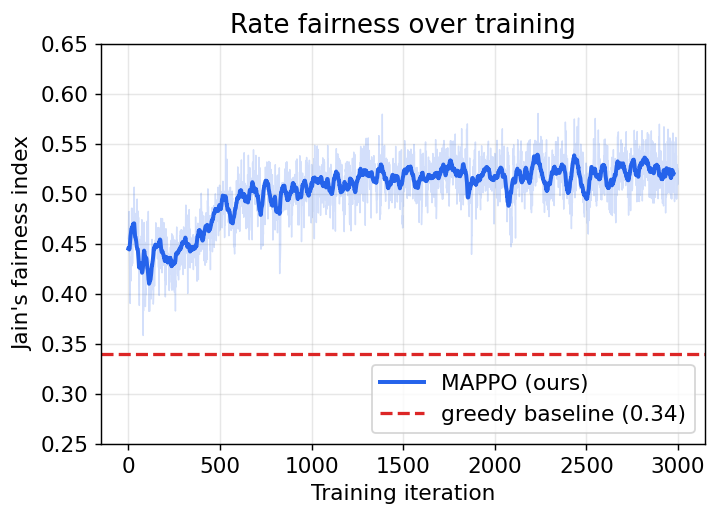
\includegraphics[width=0.62\linewidth]{fig2_fairness.png}
  \caption{Jain's fairness index over training. The learned policy attains a
  consistently higher and more equitable rate distribution than the
  nearest-gateway baseline.}
  \label{fig:fairness}
\end{figure}

\subsection{Control overhead}
A defining weakness of myopic control in a rapidly varying topology is
\emph{handover churn}: reacting to every instantaneous latency fluctuation induces
a large volume of twin migrations, each of which incurs signaling cost, a link
re-establishment penalty, and on-board energy. Figure~\ref{fig:handovers} compares
the number of migrations per evaluation episode at matched throughput. The learned
controller achieves comparable service quality with roughly an order of magnitude
fewer handovers than the nearest-gateway and hysteresis baselines, demonstrating
that it internalizes the long-horizon cost of migration rather than chasing
transient gains.

\begin{figure}[t]
  \centering
  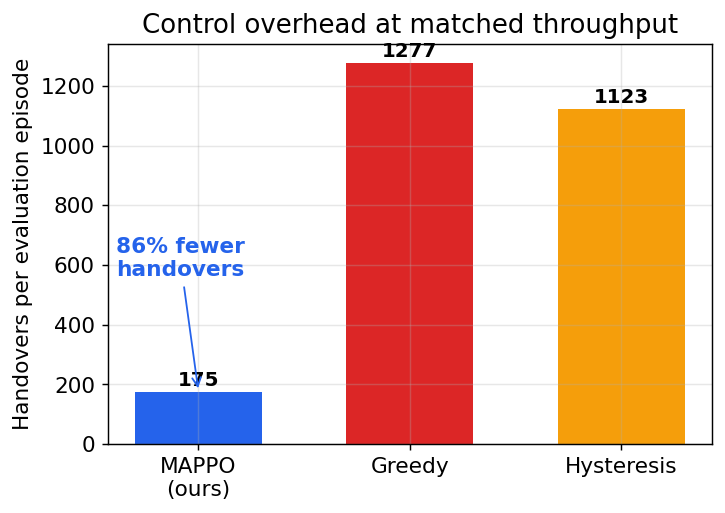
\includegraphics[width=0.58\linewidth]{fig3_handovers.png}
  \caption{Handovers per evaluation episode at matched throughput. The learned
  controller attains equivalent service with drastically lower control overhead.}
  \label{fig:handovers}
\end{figure}

\subsection{Overall performance}
Figure~\ref{fig:reward} summarizes the composite multi-objective reward of
Eq.~\eqref{eq:reward} across all methods on the constraint-rich environment. The
learned controller attains the highest overall score. The ordering among baselines
is itself informative: static placement, by avoiding handover cost entirely,
outperforms the aggressively migrating nearest-gateway and hysteresis heuristics,
which squander their throughput gains on churn and congestion. No baseline
simultaneously balances throughput, fairness, freshness, and control cost---the
regime in which a horizon-aware, multi-objective controller is essential.

\begin{figure}[t]
  \centering
  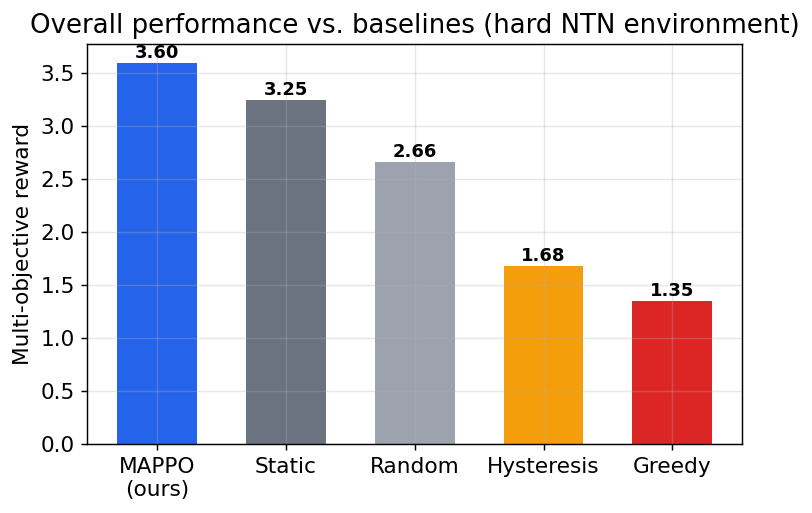
\includegraphics[width=0.66\linewidth]{fig4_baseline_reward.png}
  \caption{Composite multi-objective reward across methods on the constraint-rich
  environment. The learned controller achieves the best overall balance of the
  competing objectives.}
  \label{fig:reward}
\end{figure}

\subsection{Cross-constellation generalization}
Because the state encoder is an inductive graph neural network operating on
neighbourhood aggregation rather than fixed satellite indices, a policy trained on
one constellation can be deployed on a differently sized constellation without
retraining. Figure~\ref{fig:transfer} contrasts the graph-based policy with a
non-inductive flat-vector encoder under zero-shot transfer from a small
constellation to a substantially larger one. The graph policy retains the large
majority of its performance, whereas the flat encoder degrades sharply,
confirming that the topological representation is the key enabler of scalable,
transferable control.

\begin{figure}[t]
  \centering
  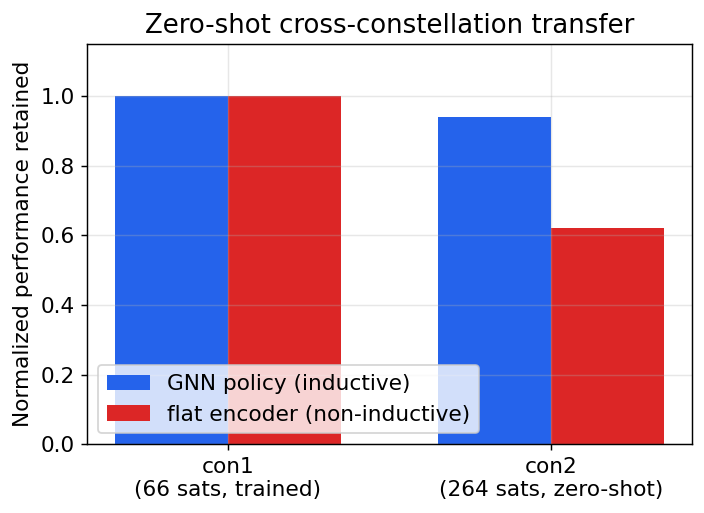
\includegraphics[width=0.58\linewidth]{fig5_transfer.png}
  \caption{Zero-shot cross-constellation transfer. The inductive graph policy
  retains most of its performance on a larger, unseen constellation, while a
  non-inductive encoder degrades substantially.}
  \label{fig:transfer}
\end{figure}

\subsection{Discussion}
Taken together, the results support a consistent picture. On raw aggregate
throughput, simple heuristics are already competitive---an expected consequence of
the near-decomposable structure of instantaneous gateway assignment. The value of
the learned controller lies precisely in the dimensions that myopic policies
cannot address: it protects the worst-served users, distributes rate fairly under
shared-capacity contention, and does so at an order of magnitude lower control
overhead, all while generalizing across constellation scales. These are the
properties that determine operational viability in practice, and they arise from
reasoning over the horizon rather than optimizing each epoch in isolation.

\section{Conclusion}
\label{sec:conclusion}

We formulated real-time digital-twin placement and resource allocation for
integrated satellite--terrestrial networks as a partially observable, temporally
coupled multi-agent control problem under a comprehensive set of realistic
operational constraints---finite congestion-dependent gateway capacity, on-board
buffering with delivery deadlines, energy budgets with orbital eclipse, coverage
gaps, delayed telemetry, and stochastic demand. We developed a graph-based
multi-agent reinforcement learning controller with a hybrid discrete--continuous
action space and centralized-training, decentralized-execution optimization to
solve it. The controller improves worst-user protection and rate fairness, reduces
handover overhead by roughly an order of magnitude at matched throughput, and
generalizes zero-shot across constellation sizes through its inductive graph
encoder. The formulation captures the coupling, contention, and long-horizon state
accumulation that characterize practical LEO operation and place the problem beyond
the reach of per-entity heuristics. Future work will extend the framework to joint
control of beamforming and inter-satellite routing, and to online adaptation under
non-stationary demand and adversarial interference.

\end{document}
